% Drift diagram of the Ornstein-Uhlenbeck model (vignette ou).
\documentclass[tikz, border = 6pt]{standalone}
\usepackage{amsmath}
\usepackage{bm}
\usetikzlibrary{arrows.meta, positioning, calc}
\tikzset{
  lat/.style = {circle, draw, thick, minimum size = 12mm, inner sep = 0pt},
  obs/.style = {rectangle, draw, thick, minimum size = 10mm, inner sep = 1pt},
  noise/.style = {circle, draw, minimum size = 7mm, inner sep = 0pt},
  reg/.style = {-{Stealth[length = 2.5mm]}, thick},
  cov/.style = {{Stealth[length = 2mm]}-{Stealth[length = 2mm]}},
  lab/.style = {font = \footnotesize, fill = white, inner sep = 1pt},
  dots/.style = {font = \Large}
}
\begin{document}
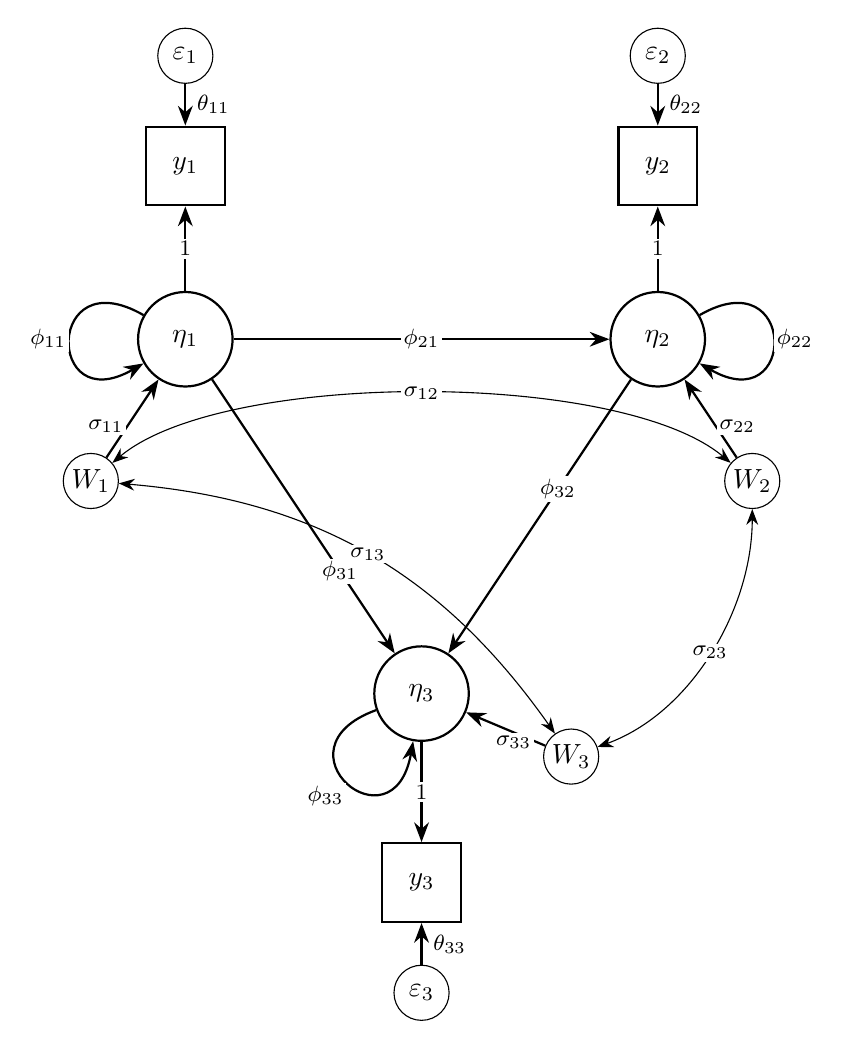
\begin{tikzpicture}
  % latent processes
  \node[lat] (e1) at (0, 0) {$\eta_{1}$};
  \node[lat] (e2) at (6, 0) {$\eta_{2}$};
  \node[lat] (e3) at (3, -4.5) {$\eta_{3}$};
  % drift: self-feedback and cross effects
  \draw[reg] (e1) to[out = 150, in = 210, looseness = 6]
    node[lab, left] {$\phi_{11}$} (e1);
  \draw[reg] (e2) to[out = 30, in = -30, looseness = 6]
    node[lab, right] {$\phi_{22}$} (e2);
  \draw[reg] (e3) to[out = 200, in = 260, looseness = 6]
    node[lab, below left] {$\phi_{33}$} (e3);
  \draw[reg] (e1) -- node[lab] {$\phi_{21}$} (e2);
  \draw[reg] (e1) -- node[lab, pos = 0.7] {$\phi_{31}$} (e3);
  \draw[reg] (e2) -- node[lab, pos = 0.4] {$\phi_{32}$} (e3);
  % process noise
  \node[noise] (w1) at (-1.2, -1.8) {$W_{1}$};
  \node[noise] (w2) at (7.2, -1.8) {$W_{2}$};
  \node[noise] (w3) at (4.9, -5.3) {$W_{3}$};
  \draw[reg] (w1) -- node[lab, pos = 0.4, left] {$\sigma_{11}$} (e1);
  \draw[reg] (w2) -- node[lab, pos = 0.4, right] {$\sigma_{22}$} (e2);
  \draw[reg] (w3) -- node[lab, pos = 0.4, below] {$\sigma_{33}$} (e3);
  \draw[cov] (w1) to[bend left = 25]
    node[lab] {$\sigma_{13}$} (w3);
  \draw[cov] (w2) to[out = -90, in = 20, looseness = 0.9]
    node[lab] {$\sigma_{23}$} (w3);
  \draw[cov] (w1) to[out = 40, in = 140, looseness = 0.6]
    node[lab] {$\sigma_{12}$} (w2);
  % measurement
  \node[obs] (y1) at (0, 2.2) {$y_{1}$};
  \node[obs] (y2) at (6, 2.2) {$y_{2}$};
  \node[obs] (y3) at (3, -6.9) {$y_{3}$};
  \node[noise] (u1) at (0, 3.6) {$\varepsilon_{1}$};
  \node[noise] (u2) at (6, 3.6) {$\varepsilon_{2}$};
  \node[noise] (u3) at (3, -8.3) {$\varepsilon_{3}$};
  \foreach \jj in {1, 2, 3} {
    \draw[reg] (e\jj) -- node[lab] {1} (y\jj);
    \draw[reg] (u\jj) -- node[lab, right = 1mm] {$\theta_{\jj\jj}$} (y\jj);
  }
\end{tikzpicture}
\end{document}
